\section{Datenbank--Schema}
\label{sec:dbschema}
\subsection{Konzeptuelles Datenbankschema: Entity--Relationship Diagramm}

Hier werden die Gegenstände der realen Welt wie in Abbildung \ref{fig:erd} gezeigt modelliert. Hierbei ist zu beachten, dass die Entität „Frage“ das zentrale Element des Datenmodells darstellt. Die weiteren Entitäten „Antwortmöglichkeit“ bzw. „gegebene Antwort” sind existenzabhängige Entities. Eine Antwortmöglichkeit kann ohne zugehörige Frage nicht existieren. Eine gegebene Antwort macht nur Sinn, wenn es eine entsprechende Antwortmöglichkeit und Frage gibt.

Die Entität „Benutzer“ steht in keiner Beziehung zu den anderen Entitäten. Sie wird auch nur für die Eingabe neuer Fragen und Antwortmöglichkeiten, bzw. zur Authentifizierung benötigt.

\begin{figure}[H]
\begin{center}
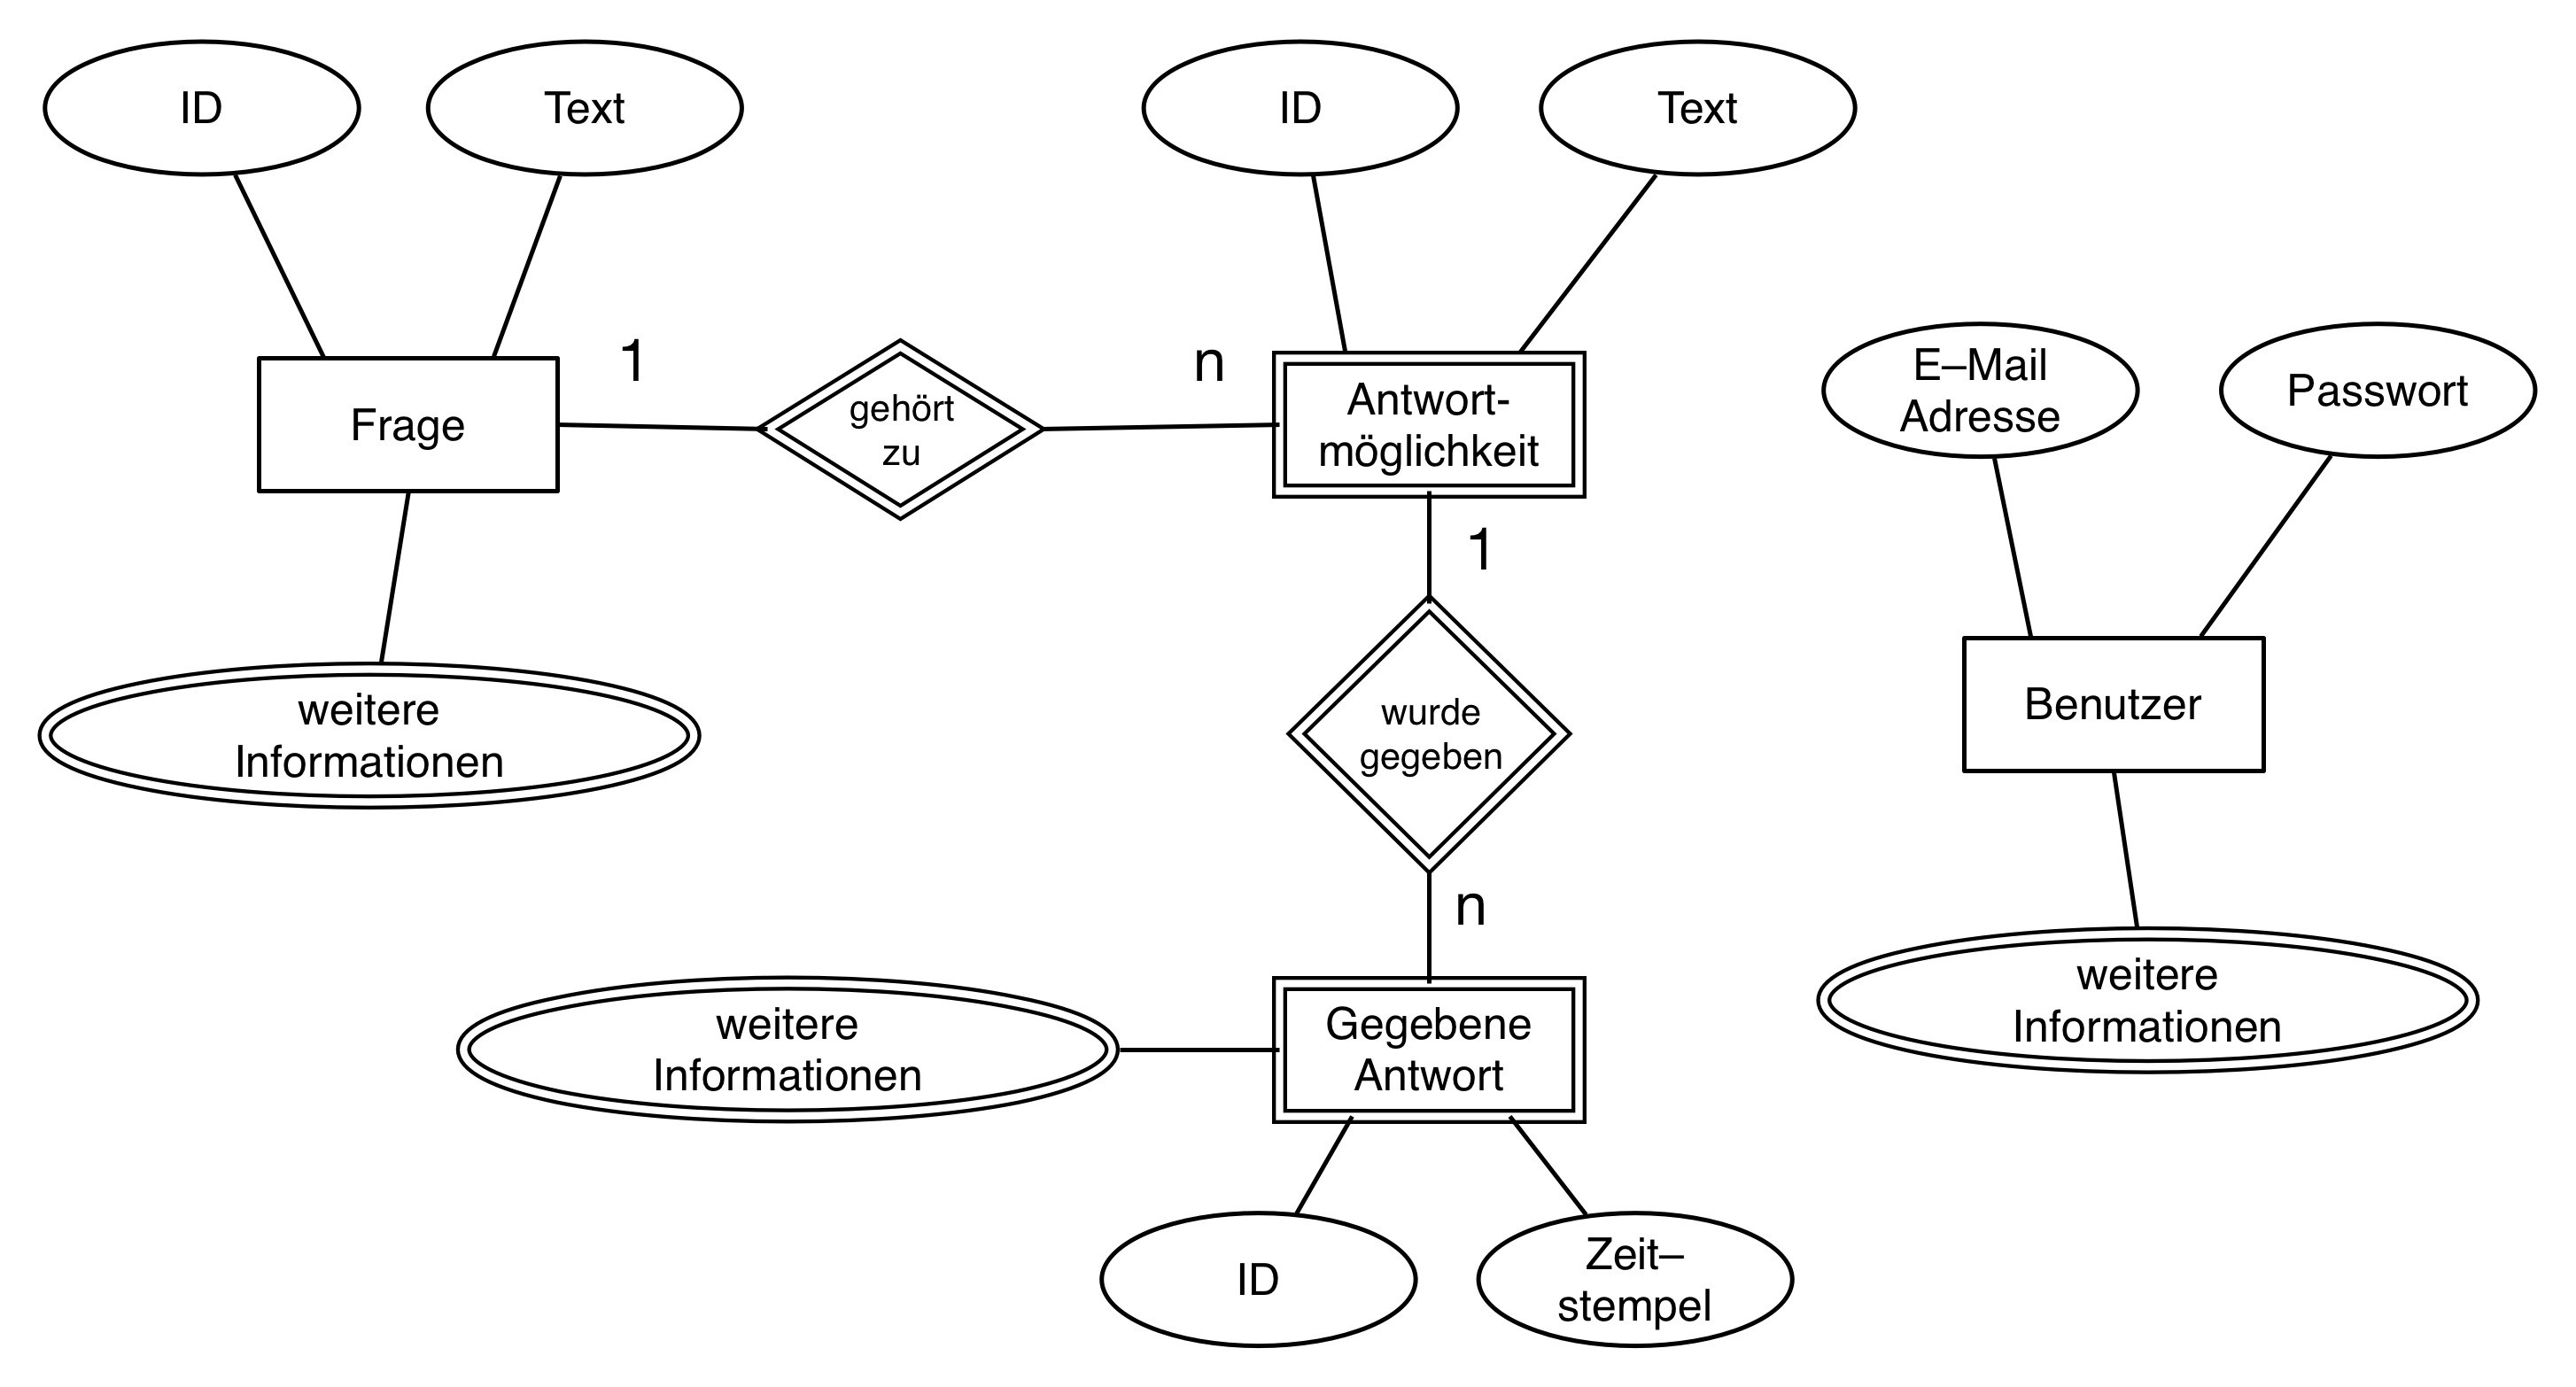
\includegraphics[width=\textwidth]{ERD.jpg}
\caption{Entity Relationship Diagram}
\label{fig:erd}
\end{center}
\end{figure}

Die als zusammengesetzte Attribute dargestellten „weiteren Informationen“ sind Attribute der jeweiligen Entitäten, die für die gestellten Anforderungen nicht notwendig sind, jedoch im Produktivbetrieb großen Zusatznutzen bieten könnten. So wäre es möglich die gegebenen Antworten durch die Speicherung der IP--Adresse, Browser--Fingerprinting\footnote{Die Identifikation eines speziellen Nutzers durch Konfigurationsdetails des Webbrowsers, Bildschirmgröße, Betriebssystemversion, etc. (siehe auch \url{https://panopticlick.eff.org/})} oder andere Techniken genauer zu identifizieren und somit einem bestimmten Nutzer zuzuordnen. Hierbei sind dann die jeweiligen Datenschutzbestimmungen zu beachten.

Die Datensätze der Entity „Frage“ könnten Zeitangaben enthalten, die festlegen, wann bzw. wie lange eine Frage auf der Website angezeigt wird. Die Antwortmöglichkeiten könnten durch entsprechende Angaben zur Sortierreihenfolge geordnet werden.

\subsection{Logisches Datenbankschema: Relationales Datenmodell}

Aufgrund des in Abbildung \ref{fig:erd} auf Seite \pageref{fig:erd} dargestellten Modell ergibt sich die in Abbildung \ref{fig:relmod} dargestellten Relationen. Dieses Modell entspricht der dritten Normalform\footnote{Kriterien laut \cite{dao101}, Kapitel 3.4}.

\begin{figure}[H]
\begin{center}
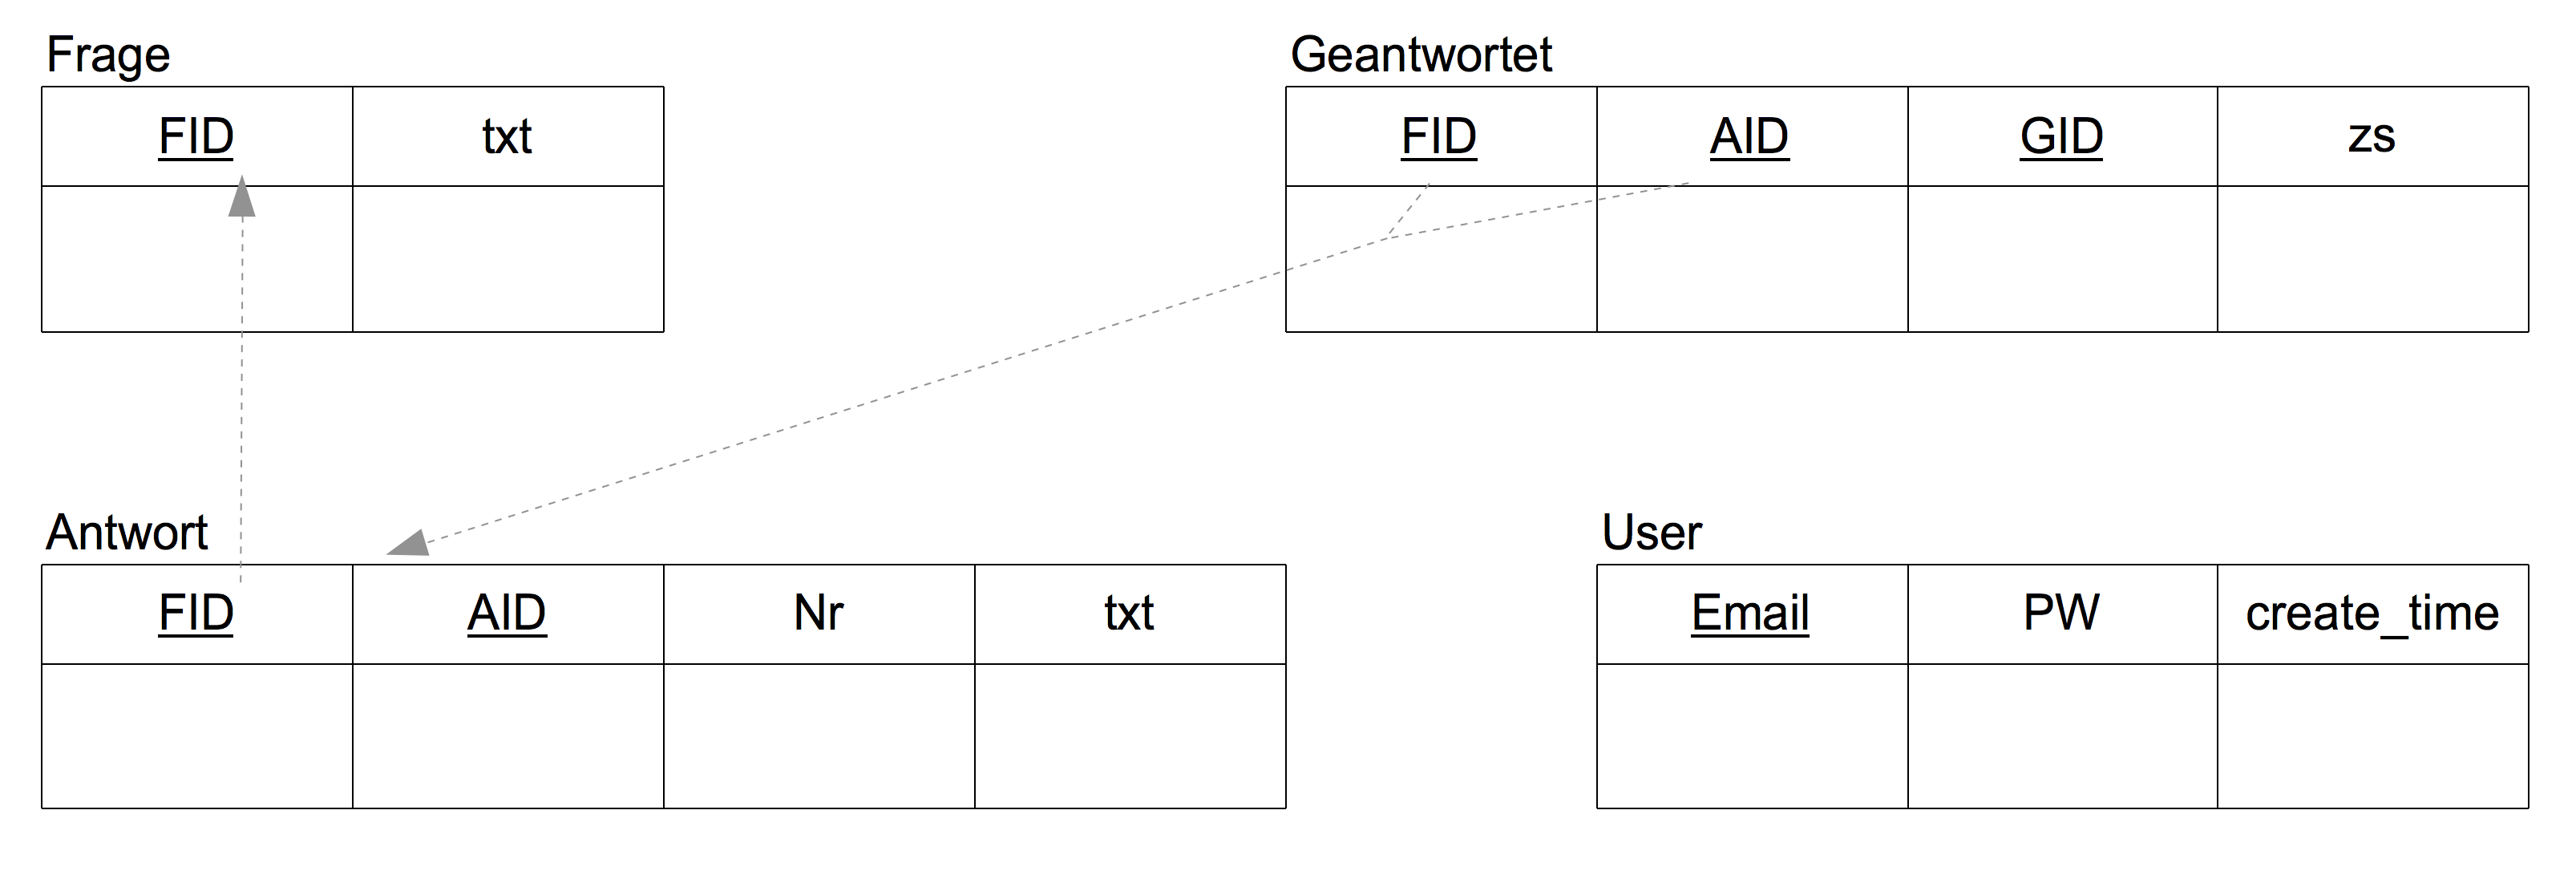
\includegraphics[width=\textwidth]{relmod.jpg}
\caption{Relationales Modell}
\label{fig:relmod}
\end{center}
\end{figure}

\subsection{Umsetzung in SQL}

\subsubsection{Tabelle: user --- Benutzerverwaltung}
\label{sec:tbluser}
\begin{figure}[H]
\begin{spacing}{1.0}
\begin{minted}[bgcolor=bg]{sql}
CREATE TABLE user (
  email VARCHAR(255) NOT NULL,
  pw CHAR(32) NOT NULL,
  create_time TIMESTAMP DEFAULT CURRENT_TIMESTAMP,
  PRIMARY KEY (`email`));
\end{minted}
\caption{SQL: CREATE TABLE user}
\label{sql:tbluser}
\end{spacing}
\end{figure}

Als Benutzername und auch als Primärschlüssel wird die E--Mail Adresse des Administrators genutzt. Da diese den Nutzer eindeutig identifiziert, wird auf einen seperaten Nutzernamen und auch auf eine generierte ID als Primärschlüssel verzichtet.

Das Passwort sollte nicht im Klartext in der Datenbank gespeichert werden. Ein \code{salted hash}\footnote{Also der Hashwert des Passworts, welches zuvor mit applikationsspezifischen Zusatzdaten ergänzt wurde} schützt hier das Passwort vor dem Ausspähen durch den Administrator selbst\footnote{Spätestens seit dem Datenklau bei Vodafone\footnote{\cite{vodafone}} eine dokumentierte Gefahr} oder durch Angreifer.\\
Die hier reservierten 32 Byte sind für den in der MySQL--Dokumentation\footnote{\cite{mysql:md5}} empfohlenen MD5-Hash ausreichend. Da die entsprechende PHP--Dokumentation\footnote{\cite{php:md5}} hier allerdings eine genau entgegengesetzte Empfehlung gibt, ist dieser Sicherheitsaspekt für ein Produktivsystem nochmals genauer zu prüfen.

\subsubsection{Tabelle: frage --- Fragestellungen}
\begin{figure}[H]
\begin{spacing}{1.0}
\begin{minted}[bgcolor=bg]{sql}
CREATE TABLE frage (
  fid INT NOT NULL AUTO_INCREMENT,
  txt VARCHAR(1024) NOT NULL,
  CONSTRAINT pk_frage PRIMARY KEY (`fid`));
\end{minted}
\caption{SQL: CREATE TABLE frage}
\label{sql:tblfrage}
\end{spacing}
\end{figure}

In der Tabelle \code{frage} wird lediglich der Text der Frage sowie die eindeutige Frage--ID gespeichert. Letztere dient als Primärschlüssel.

\subsubsection{Tabelle: antwort --- Antwortmöglichkeiten}
\begin{figure}[H]
\begin{spacing}{1.0}
\begin{minted}[bgcolor=bg]{sql}
CREATE TABLE antwort (
  fid INT NOT NULL, 
  aid INT NOT NULL AUTO_INCREMENT,
  nr  INT NULL,
  txt VARCHAR(1024) NOT NULL,
  CONSTRAINT pk_antwort PRIMARY KEY (fid, aid),
  CONSTRAINT fk_antwort_frage_fid FOREIGN KEY (fid) 
  REFERENCES frage(fid) 
  ON UPDATE CASCADE 
  ON DELETE CASCADE );
\end{minted}
\caption{SQL: CREATE TABLE antwort}
\label{sql:tblantwort}
\end{spacing}
\end{figure}

Aufgrund der Modellierung als schwache Entity setzt sich der Primärschlüssel der Tabelle \code{antwort} aus der Frage--ID sowie der Antwort--ID zusammen. Zusätzlich wird der Antworttext sowie eine frei zu vergebende Nummer gespeichert, welche für die Sortierreihenfolge bei der Anzeige genutzt werden kann.

Die Integritätsbedingung wird so definiert, dass beim Löschen einer Frage auch die zugehörigen Antwortmöglichkeiten gelöscht werden.

\subsubsection{Tabelle: geantwortet --- Gegebene Antworten}
\begin{figure}[H]
\begin{spacing}{1.0}
\begin{minted}[bgcolor=bg]{sql}
CREATE TABLE geantwortet (
  fid INT NOT NULL,
  aid INT NOT NULL,
  gid INT NOT NULL AUTO_INCREMENT,
  zs TIMESTAMP DEFAULT CURRENT_TIMESTAMP,
  CONSTRAINT pk_geantwortet PRIMARY KEY (fid, aid, gid),
  CONSTRAINT fk_geantwortet_antwort_aid FOREIGN KEY (fid, aid) 
  REFERENCES antwort(fid, aid) 
  ON UPDATE CASCADE 
  ON DELETE CASCADE );
\end{minted}
\caption{SQL: CREATE TABLE geantwortet}
\label{sql:tblgeantwortet}
\end{spacing}
\end{figure}

Für die Speicherung der gegebenen Antworten in der Tabelle \code{geantwortet} genügt der aus Frage--ID, Antwort--ID und Geantwortet--ID zusammengesetzte Primärschlüssel. Zusätzlich wird noch der jeweilige Zeitstempel für spätere Auswertungen erfasst.

Auch hier stellt die Integritätsbedingung sicher, dass beim Wegfall der entsprechenden Antwortmöglichkeit keine undefinierten gegebene Antworten zurückbleiben.
